\documentclass[fleqn]{report} 
\usepackage{amsmath, amsfonts, graphicx, adjustbox, mcode}
\begin{document}
\title{Numerical Methods 4H Assignment 1 - Adaptive Quadrature}
\author{1107023m}
\date{November 2014}
\maketitle

\section{Question 1}
Showing the error of the Simpson's rule is:
\begin{equation*}
E(f;a,b) = -\frac{(b-a)^5}{2880}f^{iv}(c), for\ some \ c \in [a,b]
\end{equation*}
Consider the Taylor expansion about the mid point $c = (a+b)/2$. 
Let $h =b-a$, then $a =c$$-h/2$ and $b=c+h/2$.

\begin{equation}
\begin{split}
f(a) & =f(c - \frac{h}{2})\\
& = f(c) - \frac{h}{2}f'(c) + \frac{h^2}{8}f''(c) - \frac{h^3}{48}f'''(c) + \frac{h^4}{384}f^{(iv)}(c) + O(h^5)
\end{split}
\end{equation}

\begin{equation}
\begin{split}
f(b) & =f(c + \frac{h}{2})\\
& = f(c) + \frac{h}{2}f'(c) + \frac{h^2}{8}f''(c) + \frac{h^3}{48}f'''(c) + \frac{h^4}{384}f^{(iv)}(c) + O(h^5)
\end{split}
\end{equation}

\begin{equation}
\begin{split}
f(x) & =f(c + (x - c))\\
& = f(c) + (x - c)f'(c) + \frac{(x-c)^2}{2!}f''(c) + \frac{(x-c)^4}{4!}f^{(iv)}(c) + O(h^5) 
\end{split}
\end{equation}

Substitute $x=c+uh/2$ into (3) and integrate (3) term by term, then

\begin{equation*}
M(f) = \int_a^b \! f(x) \, \mathrm{d}x. 
= hf(c) + \frac{h^3}{24}f''(c) + \frac{h^5}{1920}f^{(iv)}(c) + O(h^7)
\end{equation*}

Let N(f,h) be the discretization method that approximates M(f). In this case it will be Simpson's rule:

\begin{equation*}
N(f,h) = \frac{h}{6}(f(a) + 4f(c) + f(b))
\end{equation*}

Substitute (1) and (2) into N(f,h):

\begin{equation*}
\begin{split}
N(f,h) & =\frac{h}{6}[6f(c) + \frac{h^2}{4}f''(c) + \frac{h^4}{192}f^{(iv)}(c) + O(h^6)]\\
& = hf(c) + \frac{h^3}{24}f''(c) + \frac{h^5}{1152}f^{(iv)}(c) + O(h^7)
\end{split}
\end{equation*}

We can now calculate the Error E(h):

\begin{equation*}
\begin{split}
E(h) & =M(f) - N(f,h)\\
& = \frac{h^5}{1920}f^{(iv)}(c) -  \frac{h^5}{1152}f^{(iv)}(c) + O(h^7) \\
   % \text{Can discard O(h^7) as 5 < 7}\\
& = h^5f^{(iv)}(c)(\frac{1}{1920} - \frac{1}{1152})\\
& = \frac{-h^5f^{(iv)}(c)}{2880}\\
& = \frac{-(b-a)^5f^{(iv)}(c)}{2880}
\end{split}
\end{equation*}

as required.

\pagebreak



\section{Question 2}
Deriving Simpsons' Composite Rule\\

We'll generate N equal sub-intervals of [a,b], for some N $\in \mathbb{N}$\\
Label the sub-intervals as $I_{i}$ with end-points $[x_{2i-2}, x_{2i}]$, for i = 1,...,N\\
The intervals are of equal length $x_{2i} - x_{2i-2} = 2h = \frac{(b - a)}{N}$\\
Where there are 2N + 1 quadrature points $x_{i} = a + ih,$ i = 0,...,2N\\

Then the simpson rule on $I_{i}$ is:

\begin{equation*}
\begin{split}
\int_{I_i} \! f(x) \, \mathrm{d}x. & = \frac{2h}{6}
(f(x_{2i-2}) + 4f(\frac{x_{2i-2} + x_{2i}}{2}) + f(x_{2i}))\\
& = \frac{h}{3}(f(x_{2i-2}) + 4f(x_{2i-1}) + f(x_{2i}))
\end{split}
\end{equation*}

and the sum of integrals over the sub-intervals is:

\begin{equation*}
\begin{split}
\int_a^b \! f(x) \,\mathrm{d}x. & \approx  \sum_{i=1}^{N} \int_{I_i} \! f(x) \,\\
& = \sum_{i=1}^{N} \frac{h}{3}(f(x_{2i-2}) + 4f(x_{2i-1}) + f(x_{2i}))\\
& = \frac{h}{3} \sum_{i=1}^{N} (f(x_{2i-2}) + 4f(x_{2i-1}) + f(x_{2i}))\\
& = \frac{h}{3} (f(x_0) + f(x_{2N}) +  2\sum_{i=1}^{N-1} f(x_{2i}) + 4\sum_{i=1}^{N} f(x_{2i-1}))
\end{split}
\end{equation*}    

\pagebreak

\section{Question 3}
Deriving the error in the Composite Simpson's rule $S_c(f;a,b,N)$
\begin{equation*}
E_c(f;a,b,N) = -\frac{(b-a)^5}{2880N^4}f^{iv}(c),\ for \ some \ c \in [a,b]
\end{equation*}

\noindent It is not possible to derive the Composite Simpsons' error with only
the information on the error for the normal Simpsons' rule. The Composite
Simpson's rule performs the Simpson's rule on multiple sub-intervals meaning the
error would be the sum of the errors of the ordinary Simpsons' rule on each sub-inverval. 
But since $f^{iv}(c)$ must be a different value of c for each interval;
there is not enough information to combine these error intervals to derive the composite error.\\

\noindent For the jth node, $x_j = a + jh, \ j \in [0, 2N]$, \\
Expanding $f(x_j)$ using the Taylor Expansion gives the following:
\begin{equation}
f(x_j) = f(a + jh) = f(a) + jhf'(a) + \frac{(jh)^2}{2!}f''(a) + \frac{(jh)^3}{3!}f'''(a) + \frac{(jh)^4}{4!}f^{(iv)}(a) + O(h^5)
\end{equation}

\noindent Let x = a + uh, then $f(x)$ gives the following Taylor Expansion:
\begin{equation}
f(x) = f(a + uh) = f(a) + uhf'(a) + \frac{(uh)^2}{2!}f''(a) + \frac{(uh)^3}{3!}f'''(a) + \frac{(uh)^4}{4!}f^{(iv)}(a) + O(h^5)
\end{equation}
Since we have 2N + 1 points, $u \in [0, 2N]$ integrating $f(x)$ gives the following:
\begin{equation}
\begin{split}
M(f) &= \int_0^{2N} \! hf(a + uh) \, \mathrm{d}u.\\ 
&= h [uf(a) + \frac{u^2h}{2}f'(a) + \frac{u^3h^2}{6}f''(a) + \frac{u^4h^3}{24}f'''(a) + \frac{u^5h^4}{120}f^{(iv)}(a) + O(h^5)]_0^{2N}\\
&= 2Nhf(a) + 2(Nh)^2f'(a) + \frac{4(Nh)^3}{3}f''(a) + \frac{2(Nh)^4}{3}f'''(a) + \frac{4(Nh)^5}{15}f^{iv}+ O(h^6)
\end{split}
\end{equation}

\noindent To solve for $E_c(f;a,b,N)$ we note that 
\begin{equation*}
S_c(f;a,b,N) = \frac{h}{3} (f(x_0) + f(x_{2N}) +  2\sum_{i=1}^{N-1} f(x_{2i}) + 4\sum_{i=1}^{N} f(x_{2i-1}))
\end{equation*}
substitute each term into the $f(xj)$ expansion (4), and then subtract the whole sum from
M(f). This should result in the error value.

\pagebreak

\section{Question 4}
Implementation of Composite Simpsons' rule in Matlab. \\

See file Sc.matlab for the same code as below.

\lstinputlisting[language=Matlab, frame=single]{Sc.matlab}

\pagebreak

\section{Question 5}
Considering an interval [a,b] small enough to justify $f^{iv}(x) = const$ on [a,b] Prove: 
\begin{equation*}
E(f;a,b,2) = \frac{1}{15}(S_c(f;a,b,2) - S_c(f;a,b,1))\ and\ then\ \int_a^b \! f(x) \, \mathrm{d}x  = S_c(f;a,b,2) + E(f;a,b,2)
\end{equation*}

\noindent Solution: \\

\noindent Note that:

\begin{equation*}
\begin{split}
Sc(f;a,b,1) &= \frac{h}{3} (f(x_0) + f(x_{2}) +  2\sum_{i=1}^{0} f(x_{2i}) + 4\sum_{i=1}^{1} f(x_{2i-1}))\\
            & = \frac{h}{3} (f(x_0) + 4f(x_1) + f(x_2))\\
            & = \frac{h}{3} (f(a) + 4f(\frac{a + b}{2}) + f(b))\\
            & = S(f;a,b)\\
\end{split}
\end{equation*}

\begin{equation*}
\implies Ec(f;a,b,1) = E(f;a,b)
\end{equation*}


\noindent As $f^{iv}$ is constant: $f^{(iv)}(c) = \alpha$ for $ \forall c \in [a,b]$ 
where $\alpha$ is a constant\\ 
Then:

\begin{equation*}
E(f;a,b) = -\frac{(b - a)^5}{2880}\alpha
\end{equation*}

\begin{equation*}
E_c(f;a,b,2) = -\frac{(b - a)^5}{2880 * 2^4}\alpha
\end{equation*}

\begin{equation*}
\implies E(f;a,b) = 16E_c(f;a,b,2)
\end{equation*}


\noindent Let $M(f) = \int_a^b \! f(x) \, \mathrm{d}x$ \\

From definition of Numerical Schemes

\begin{equation*}
\begin{split}
&M(f) = S_c(f;a,b,2) + E_c(f;a,b,2)\\
&M(f) = S_c(f;a,b,1) + E_c(f;a,b,1)
\end{split}
\end{equation*}


Then:

\begin{equation*}
\begin{split}
S_c(f;a,b,2) - S_c(f;a,b,1) & = M(f) - E_c(f;a,b,2) - M(f) + E_c(f;a,b,1)\\
& = E_c(f;a,b,1) - E_c(f;a,b,2)\\
& = E(f;a,b) - E_c(f;a,b,2)\\
& = 16E_c(f;a,b,2) - E_c(f;a,b,2)\\
& = 15E_c(f;a,b,2)\\
\end{split}
\end{equation*}

\begin{equation*}
\iff \frac{1}{15}(S_c(f;a,b,2) - S_c(f;a,b,1)) = E_c(f;a,b,2)
\end{equation*}

as required.\\

\noindent Let $E(f;a,b,2) = E_c(f;a,b,2)$ and by $M(f) = S_c(f;a,b,2) + E_c(f;a,b,2)$ 
it follows that:\\

\begin{equation*}
\int_a^b \! f(x) \, \mathrm{d}x  = S_c(f;a,b,2) + E(f;a,b,2)
\end{equation*}
\\


\pagebreak

\section{Question 6}
Implementation of Adaptive Simpsons' rule in Matlab. \\

See file Sa.matlab for the same code as below.

\lstinputlisting[language=Matlab, frame=single]{Sa.matlab}

\pagebreak

\section{Question 7}

Plotting $ \int_0^2 \! sin(1 - 25erf(\frac{x-1}{0.2\sqrt{2}}) \,\mathrm{d}x.$ 
at first with the adaptive simpsons rule with an error of $10^{-3}$ is evaluated at 
133 unique points. Then plotting the same amount of points with 66 intervals of composite 
simpson's rule gives the following graphs for each. The '+' marks the points at which
the function is evaluated at.

\begin{figure}[h!]
\begin{center}
    \centerline{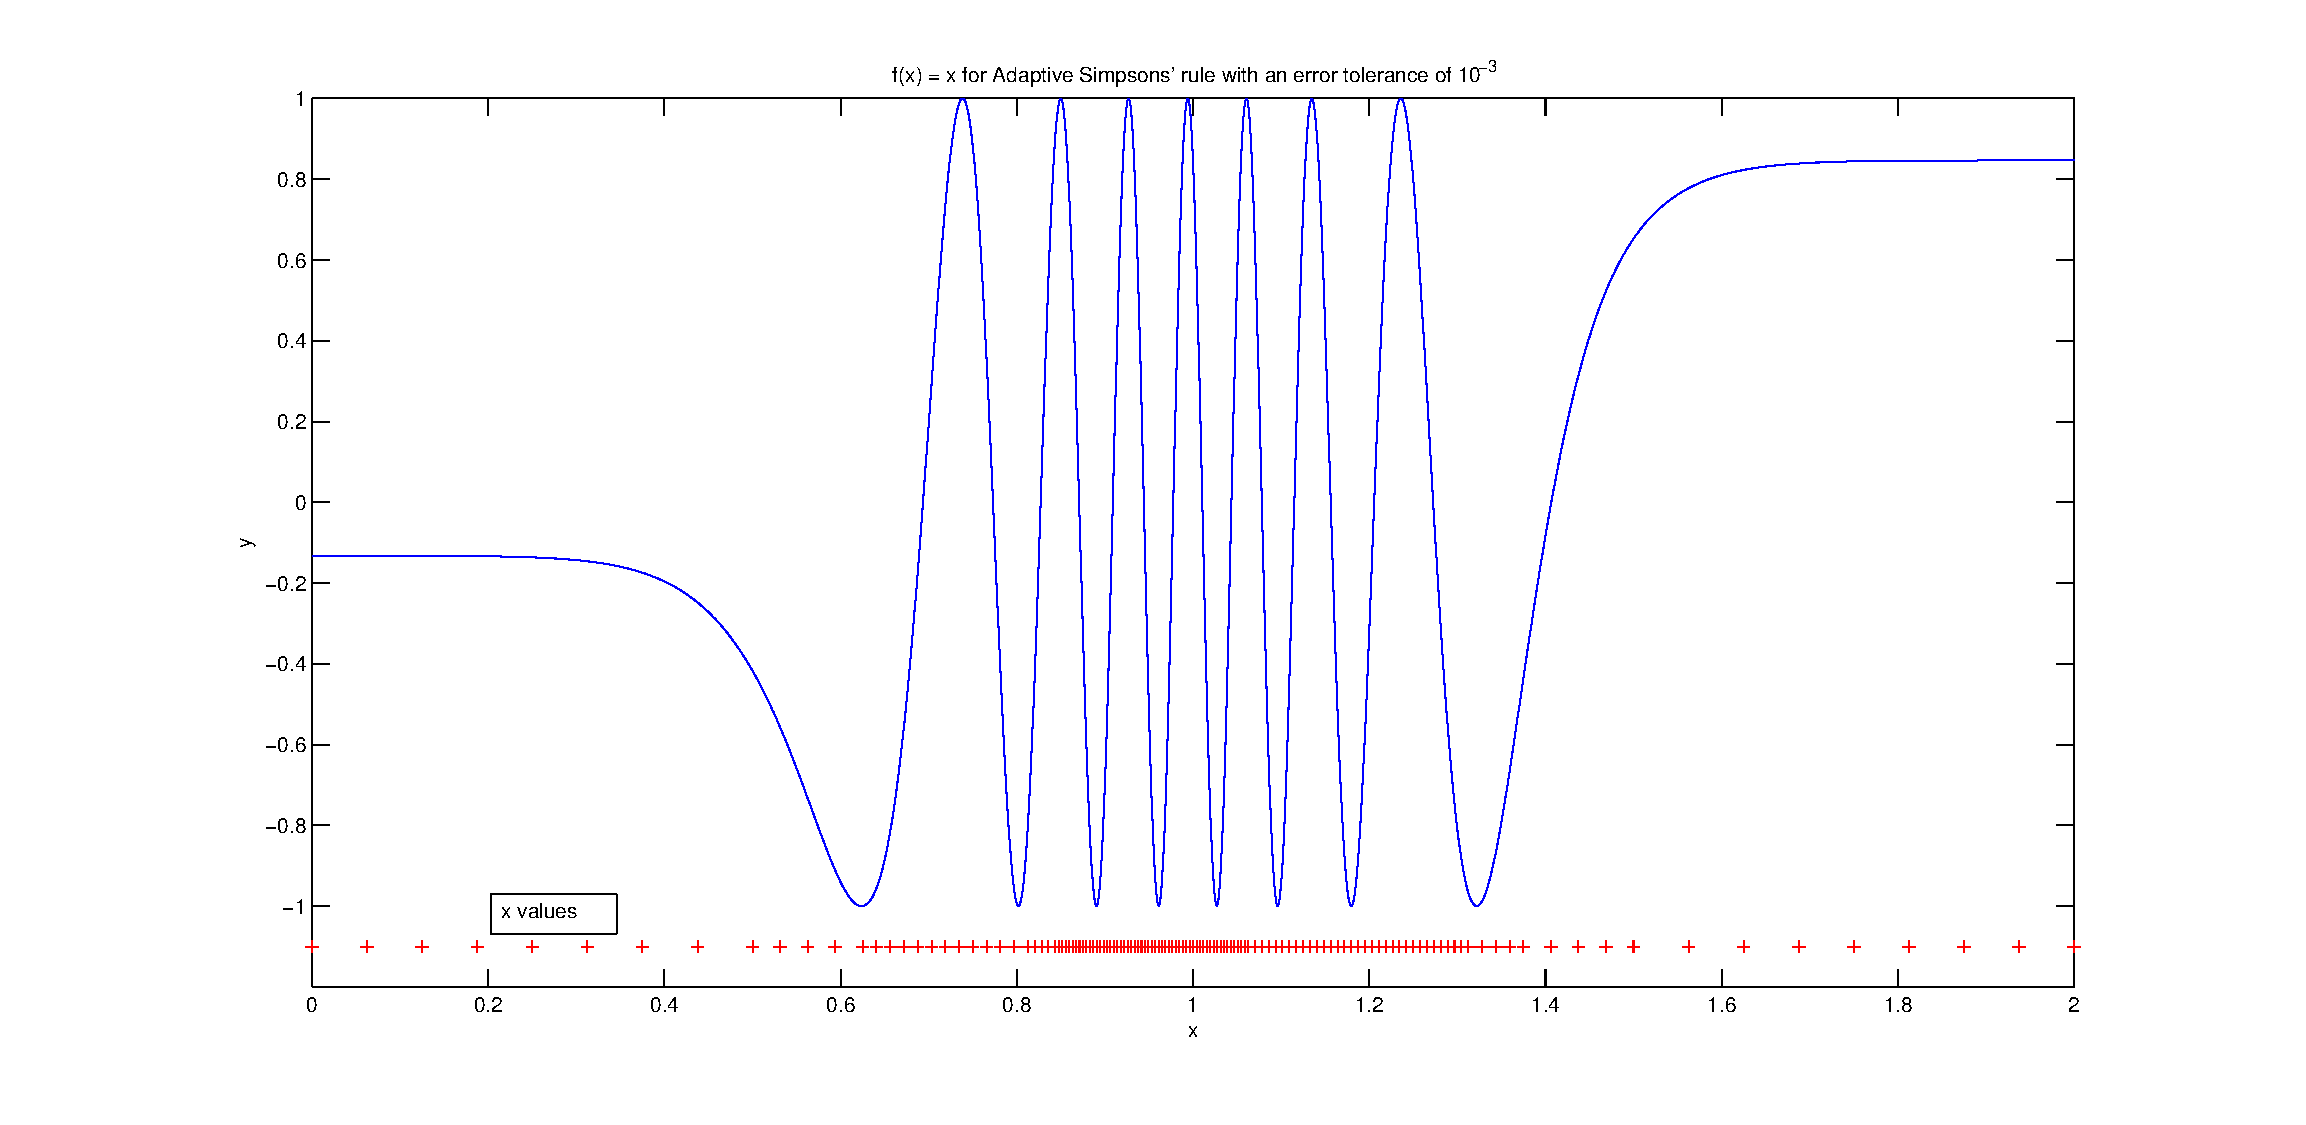
\includegraphics[width=1.8\textwidth]{graphs/q7adaptive.eps}}
    \caption{Adaptive Simpsons'}
\end{center}
\end{figure}

\pagebreak

\begin{figure}[h!]
\begin{center}
    \centerline{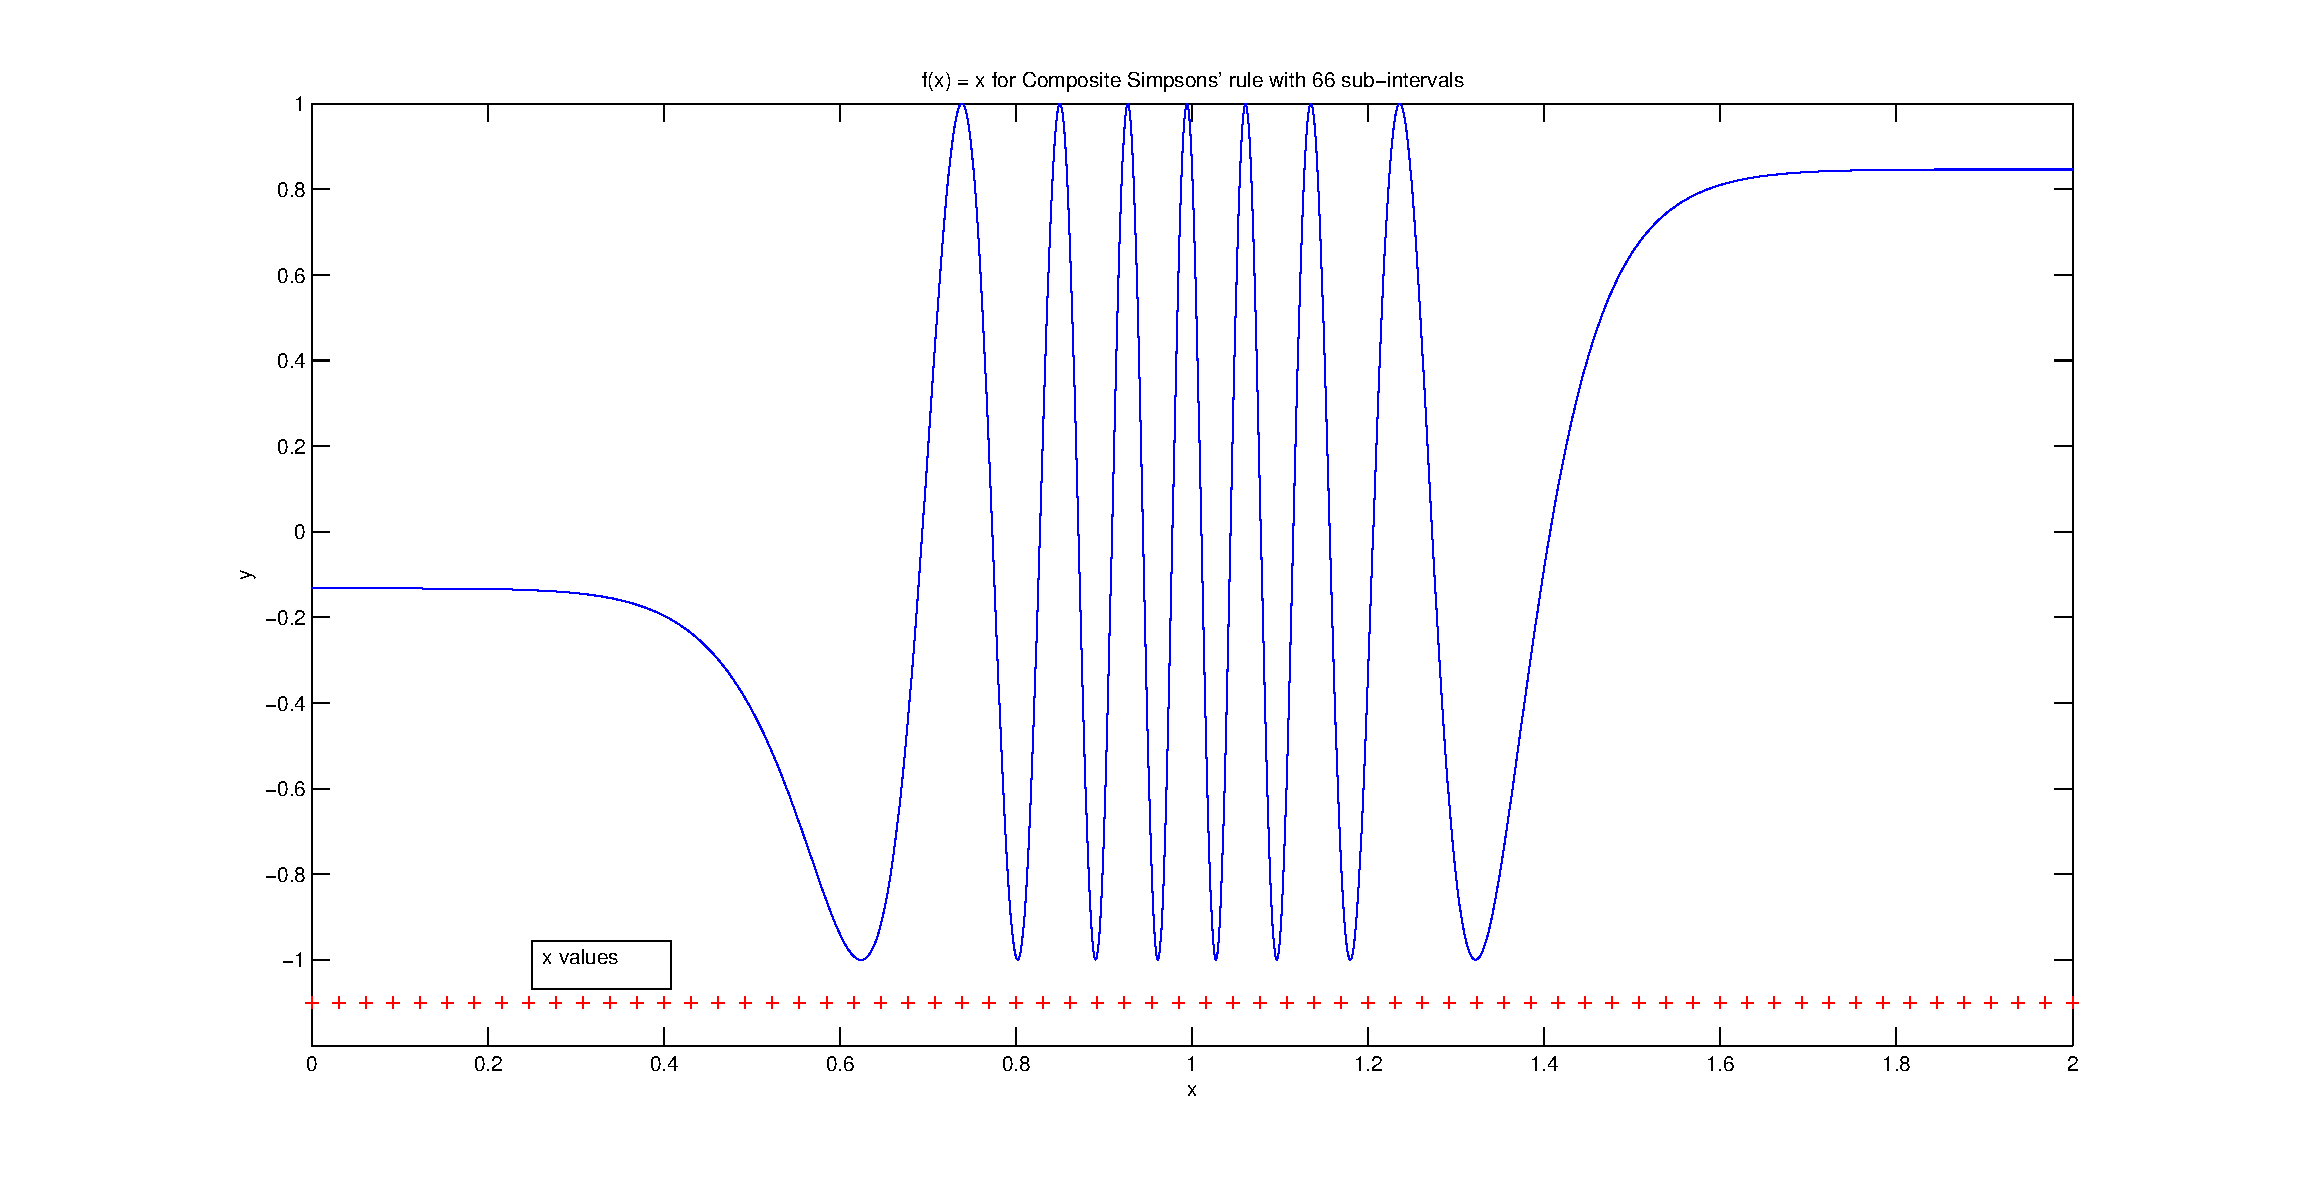
\includegraphics[width=1.8\textwidth]{graphs/q7composite.eps}}
    \caption{Composite Simpson'}
\end{center}
\end{figure}

As you can see for the Composite Simpsons' rule, the quadrature points 
are uniform. Whereas for the Adaptive Simpsons' rule the quadrature points
are more around the centre. This makes sense as the error
is likely to be larger where the graph isn't as `regular`, so the
adaptive procedure tends towards those intervals.

\pagebreak

\section{Question 8}

Plotting $ \int_0^2 \! sin(1 - 25erf(\frac{x-1}{0.2\sqrt{2}}) \,\mathrm{d}x.$ 
For the integral 

\begin{equation*}
I = \int_{-3}^5 \! exp(-50(x-1)^{2}) \,\mathrm{d}x.
\end{equation*}

Taking 10 equally spaced error tolerance values ranging from $10^-6$ to $10^-12$
and applying them to the Adaptive Simpsons' function then working out
absolute value of the difference between the results and the actual values; and applying
this against the error tolerance values supplied gives the following graph:

\newpage

\begin{figure}[h!]
\begin{center}
    \centerline{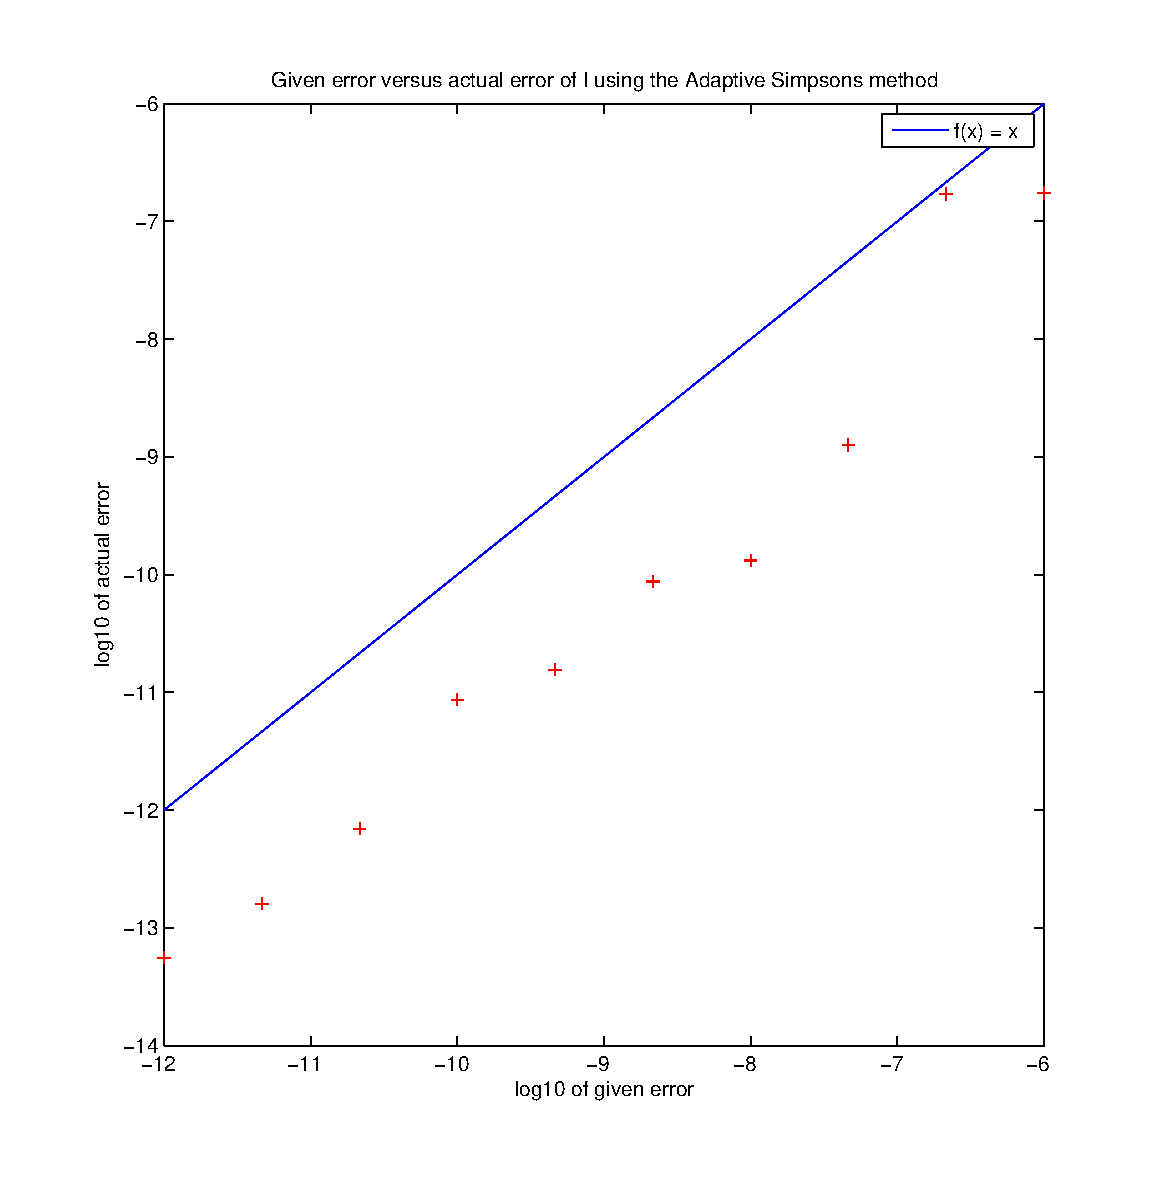
\includegraphics[width=1.4\textwidth]{graphs/q8.eps}}
    \caption{Adaptive Error'}
\end{center}
\end{figure}

The graph shows as expected as the Adaptive Simpsons' formula should give an error of equal to
or less than that given to it. Which can be seen for all 10 points on the graph. 

\end{document}
